\documentclass{article}
\usepackage{graphicx} % Required for inserting images
\documentclass{article}
\usepackage{amsmath}
\usepackage{amssymb}
\usepackage[utf8]{inputenc}
\usepackage{amsmath}
\usepackage{amssymb}
\usepackage{authblk}
\usepackage{setspace}
\usepackage[margin=1.25in]{geometry}
\usepackage{graphicx}
\graphicspath{ {./figures/} }
\usepackage{subcaption}
\usepackage{amsmath}
\usepackage{lineno}
\usepackage{hyperref}
\usepackage{comment}
\usepackage{lipsum}
\usepackage{physics}


\usepackage{xcolor}

\newcommand{\highlight}[1]{%
  \colorbox{red!50}{$\displaystyle#1$}}


\usepackage[style=nejm, 
citestyle=numeric-comp,
sorting=none]{biblatex}
\addbibresource{PartIIIProjectTemplate.bib}


\title{Project Progress Notebook}
\author{PRABHODA C S}
\date{December 2024}

\begin{document}

\maketitle

\section{Variable translation from Salvio to Barker}  \label{Section 1}
Silvio \cite{Salvio_2022} and especially \cite{Pradisi_2022}, give us for the potential

\begin{equation}
    U(\omega) = \frac{1}{4 c'} \left[ \frac{M_{p}^{2}}{4} \text{sinh}(\text{X}(\omega)) - \beta  \right]^2
\end{equation}
where
\begin{equation}
    \text{X}(\omega) = \sqrt{\frac{2}{3}} \frac{\omega}{M_{p}} + \text{tanh}^{-1} \left(\frac{4 \beta}{\sqrt{M_{p}^{4}+16 \beta^2}} \right)
\end{equation}

Differentiating $U(\omega)$ and setting it equal to zero gives us that 

\begin{equation}
    \omega_{min} = \sqrt{\frac{2}{3}} M_p \left[ \text{sinh}^{-1}\left(\frac{4\beta}{M_{p}^{2}}\right) - \text{tanh}^{-1}\left(\frac{4\beta}{\sqrt{M_{p}^{4} + 16\beta^2}}\right) \right]
\end{equation}

Inserting $\text{ArcSinh(x)} = \ln(x + \sqrt{x^2 + 1})$ and $\text{ArcTanh(x)} = \frac{1}{2} \ln\left(\frac{1+x}{1-x}\right)$, gives us $\omega_{min} = 0$ always.
\\
Barker \cite{barker2024poincaregaugetheoryconformal} gives us potential

\begin{equation}
    U(\varphi) = \frac{\mu^2 \phi_{0}^{4}}{2} \left[ \frac{\sigma}{2} + \sqrt{\nu - \frac{\sigma^2}{4}} \text{sinh}\left( \text{X}(\varphi) \right)  \right]
\end{equation}
where
\begin{equation}
    \text{X}(\varphi) =  \frac{\varphi}{\phi_0 \sqrt{\nu - \frac{\sigma^2}{4}}} - \frac{c}{\phi_0 \sqrt{\nu - \frac{\sigma^2}{4}}}
\end{equation}

\subsection{Translating Variables}   \label{Section 1.1}
We know that, $[\beta] = [M_{p}^{2}]$  and $[c'] = 0$ from \cite{Pradisi_2022}. If we want $\varphi = \omega$ (it can't be $\varphi = f(\omega)$ as that would ruin the $(\partial\varphi)^2$ term in Lagrangian), we are forced to make the substitutions that make dimensional sense:

\begin{align}
    \phi_0 &= \sqrt{\frac{3}{2}} M_p \label{eq:A} \\
    \mu &= \frac{1}{6 \sqrt{2 c'}} \label{eq:B} \\
    \sigma &= -\frac{8 \beta}{M_{p}^{2}} \label{eq:C} \\
    \nu &= 1 + \frac{16 \beta^2}{M_{p}^{4}} \label{eq:D} \\
    c  &= -\sqrt{\frac{3}{2}} M_{p} \text{tanh}^{-1} \left(\frac{4 \beta}{\sqrt{M_{p}^{4}+16 \beta^2}} \right) \label{eq:E}
\end{align}

Now, $[\phi_0] = [c] = [M_p]$ and the rest, $[\mu] = [\sigma] = [\nu] = 0$, to be fair, we can include a term $g^{-1}$ in front of the sinh term in $\text{X}(\omega)$, s.t., $[g] = 0$, the resulting eqns are:

\begin{align}
    \phi_0 &= g \sqrt{\frac{3}{2}} M_p \label{eq:A} \\
    \mu &= g^{-1} \frac{1}{6 \sqrt{2 c'}} \label{eq:B} \\
    \sigma &= - g^{-1} \frac{8 \beta}{M_{p}^{2}} \label{eq:C} \\
    \nu &= g^{-2} \left( 1 + \frac{16 \beta^2}{M_{p}^{4}} \right) \label{eq:D} \\
    c  &= -\sqrt{\frac{3}{2}} M_{p} \text{tanh}^{-1} \left(\frac{4 \beta}{\sqrt{M_{p}^{4}+16 \beta^2}} \right) \label{eq:E}
\end{align}

We can see that in \ref{eq:A}, the field $\varphi$ has no dependence on any parameter/is not free, but is fixed by the Planck mass (in Planck units, it is 1.225).

What we can see from equations \ref{eq:A} to \ref{eq:E}, is that $\phi_0 \propto M_p$, with the constant $g$ dictating what fraction of $M_p$,  $\phi_0$ is. $\mu$ is fixed by the strength of coupling of the $\mathcal{R'}^2$ term ($c'$) in the \cite{Pradisi_2022} paper. $c$ is now no longer free and based on the results from \ref{Section 1}, we see that the minima of the potential must now always stay at $\phi_{min} = 0$.

Below is a plot of the aligned graphs with $M_p = 1$ and the values of the parameters upon translation labelled. $g = \sqrt{\frac{1}{3}}$ so that $\phi_0 < M_p$ also.

\begin{figure}[h!]
    \centering
    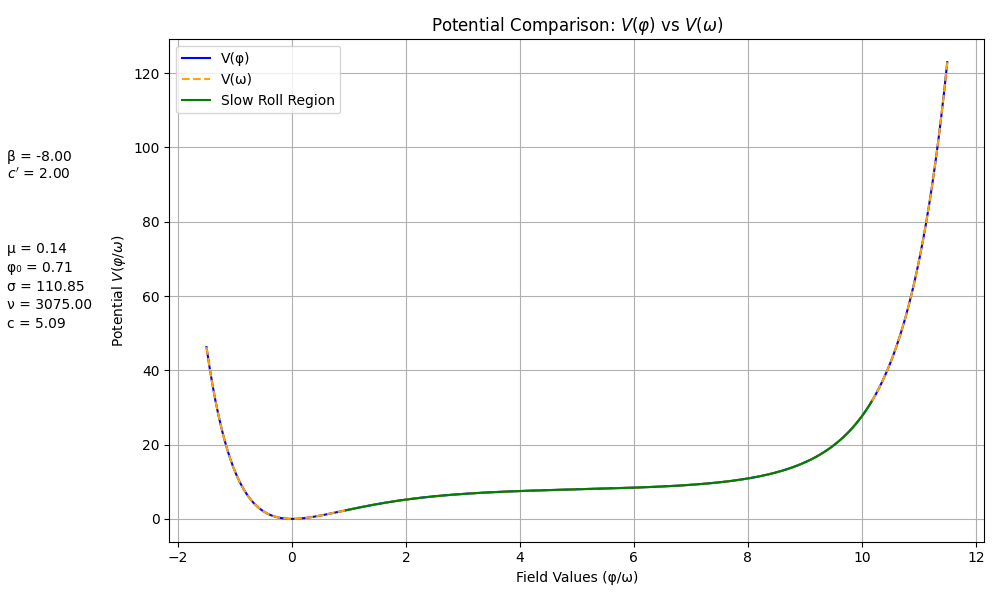
\includegraphics[width=1\textwidth]{Python/Figures/Comparing Silvio - Barker.png}
    \caption{Aligned graphs with parameter values on the side}
    \label{Aligned Potential}
\end{figure}



For this value of $\beta$, we get $N = 73.582$ as the number of e-folds.

\newpage

\newpage
\section{Coupling to gravity}


To find invariant form of Ricci scalar, look at Christoffel symbol. Can be offset by defining


\begin{equation}
    \mathcal{T}^{\alpha}_{\beta \gamma} = \Gamma^{\alpha}_{\beta \gamma} + (\delta^{\alpha}_{\beta} B_{\gamma} + \delta^{\alpha}_{\gamma} B_{\beta} - g_{\beta \gamma}g^{\alpha \tau}B_{\tau})
\end{equation}

where $B_{\mu} \rightarrow B_{\mu} - \partial_{\mu} \rho$ under a conformal transformation like in \cite{barker2024poincaregaugetheoryconformal}, 

Using this new conformally covariant connection in the definition of the Riemman tennsor and contracting to get conformally covariant Ricci Scalar (CCRS), we get 


\begin{equation}
    \tilde{R} = R - 6 B_{\mu} B^{\mu} - 6 \nabla_\mu B^\mu
\end{equation}

Under a conformal transformation $g_{\mu\nu} \rightarrow e^{2\rho}g_{\mu\nu}$, $\tilde{R} \rightarrow e^{-2\rho} \tilde{R}$
So lagrangian is ? ? 

Literature is out! Since mass scale $\phi$ (Compensator scalar) introduces fundamental scale (as seen in prev section \ref{Section 1.1}, $\phi_0 \sim M_p$), maybe first couple it directly to CCRS, gives us an action in the Jordan Frame, then, transform to Einstein frame, and then minimally couple to inflaton field $\varphi$ in the PHYSICAL Einstein Frame?

\begin{equation}
    \mathcal{L} = (\alpha \phi^2 + \beta \varphi^2 + \gamma \phi \varphi) \tilde{R} + \frac{\epsilon}{2} D_{\mu}\varphi D^{\mu}\varphi + \frac{\sigma}{2} D_{\mu}\varphi D^{\mu}\phi  +  \frac{\nu}{2} D_{\mu}\phi D^{\mu}\phi - \frac{\mu^2}{2} \phi^2 \varphi^2 - \frac{\xi}{16} H_{\mu\nu}H^{\mu\nu}
\end{equation}

\begin{equation}
    \begin{aligned}
        \mathcal{L} = &\; (\alpha \phi^2 + \beta \varphi^2 + \gamma \phi \varphi)R - 6((\alpha \phi^2 + \beta \varphi^2 + \gamma \phi \varphi)(B_{\mu} B^{\mu} + \nabla_\mu B^\mu) \\
        & +\frac{\epsilon}{2} D_{\mu}\varphi D^{\mu}\varphi + \frac{\sigma}{2} D_{\mu}\varphi D^{\mu}\phi + \frac{\nu}{2} D_{\mu}\phi D^{\mu}\phi \\
        & - \frac{\mu^2}{2} \phi^2 \varphi^2 - \frac{\xi}{16} H_{\mu\nu}H^{\mu\nu}
    \end{aligned}
\end{equation}


Taking a leaf out of \cite{barker2024poincaregaugetheoryconformal}, we pick a gauge choice $g_{\mu \nu} \rightarrow \frac{\phi_0}{\phi} g_{\mu \nu}$, $\varphi \rightarrow \frac{\phi}{\phi_0} \varphi$ and $B_{\mu} \rightarrow B_{\mu} - \partial_{\mu} ln(\phi)$. So that, the resulting action (still in jordan frame)

\begin{equation}
    \begin{aligned}
        \mathcal{L} &= (\alpha \phi^2_0 + \beta \varphi^2 + \gamma \phi_0 \varphi) (R - 6B_{\mu} B^{\mu} - 6\nabla_\mu B^\mu) \\
        &+ \frac{\epsilon}{2} (\partial_\mu \varphi - (\varphi + \frac{\sigma}{\epsilon} \phi_0)B_\mu)(\partial^\mu \varphi - \varphi B^\mu)\\
        &- \frac{\mu^2}{2} \phi^2_0 \varphi^2 + \frac{\nu \phi_{0}^{2}}{2} B_\mu B^\mu - \frac{\xi}{16} H_{\mu\nu}H^{\mu\nu}
    \end{aligned}
\end{equation}

Assuming $\xi << 1$ again or other conditions based on the result, we solve for the Euler-Lagrange Equations for field $B_\mu$ and get:

\begin{equation}
    B_\mu = \frac{1}{2} \partial_\mu \text{ln}(\epsilon \varphi^2 + \sigma \phi_0 \varphi + \nu \phi^2_0 -12 (\alpha \phi^2_0 + \beta \varphi^2 + \gamma \phi_0 \varphi))
\end{equation}

That is.

\begin{equation}
    B_\mu = \frac{1}{2} \partial_\mu \text{ln}((\epsilon - \beta') \varphi^2 + (\sigma - \gamma') \phi_0 \varphi + (\nu - \alpha')\phi^2_0)
\end{equation}


Where, $\alpha' = 12\alpha, \beta' = 12\beta \text{ and } \gamma' = 12 \gamma$

Now inputting that value of $B_\mu$ into the action and plugging through the calculations, we get

\begin{equation}
    \begin{aligned}
        S &= \int \text{d}^4\text{x} \sqrt{-g} [ (\alpha \phi^2_0 + \beta \varphi^2 + \gamma \phi_0 \varphi) R \\
          & - 6 (\alpha \phi^2_0 + \beta \varphi^2 + \gamma \phi_0 \varphi)B_{\mu} B^{\mu} + 6\partial_\mu (\alpha \phi^2_0 + \beta \varphi^2 + \gamma \phi_0 \varphi)B^\mu \\
        &+ \frac{\epsilon}{2} (\partial_\mu \varphi - (\varphi + \frac{\sigma}{\epsilon} \phi_0)B_\mu)(\partial^\mu \varphi - \varphi B^\mu)\\
        &- \frac{\mu^2}{2} \phi^2_0 \varphi^2 + \frac{\nu \phi_{0}^{2}}{2} B_\mu B^\mu - \frac{\xi}{16} H_{\mu\nu}H^{\mu\nu} ] 
    \end{aligned}
\end{equation}
So only the coefficent of the derivative becomes:
\begin{align}
    &\frac{48 \alpha  \epsilon  \phi ^2+576 \beta ^2 \varphi ^2+576 \beta  \gamma  \varphi  \phi -48 \beta  \sigma  \varphi  \phi -48 \beta  \varphi ^2 \epsilon +144 \gamma ^2 \phi ^2-24 \gamma  \sigma  \phi ^2+\sigma ^2 \phi ^2-4 \nu  \epsilon  \phi ^2}{4 \left(12 \alpha  \phi ^2+12 \beta  \varphi ^2+12 \gamma  \varphi  \phi -\nu  \phi ^2-\sigma  \varphi  \phi -\varphi ^2 \epsilon \right)} \nonumber \\
    &\implies \frac{48 \beta  \left(12 \alpha  \phi ^2+12 \beta  \varphi ^2+12 \gamma  \varphi  \phi -\nu  \phi ^2-\sigma  \varphi  \phi -\varphi ^2 \epsilon \right)+\phi ^2 \left((12 \gamma -\sigma )^2-4 (\nu -12 \alpha ) (\epsilon -12 \beta )\right)]}{4[(\epsilon - 12\beta) \varphi^2 + (\sigma - 12\gamma) \phi_0 \varphi + (\nu - 12\alpha)\phi^2_0)]} \nonumber \\
    &\implies - 12\beta + \frac{\phi_0^2 \left((12 \gamma -\sigma )^2-4 (\nu -12 \alpha ) (\epsilon -12 \beta )\right)}{4[(\epsilon - 12\beta) \varphi^2 + (\sigma - 12\gamma) \phi_0 \varphi + (\nu - 12\alpha)\phi^2_0)]}
\end{align}
becomes

\begin{equation} \label{24}
    \begin{aligned}
        S &= \int \text{d}^4\text{x} \sqrt{-g} [ (\alpha \phi^2_0 + \beta \varphi^2 + \gamma \phi_0 \varphi) R \\
        &- 12 \beta \left[ 1 - \frac{\phi_0^2}{48\beta V} [(\sigma - 12\gamma)^2 - 4(\epsilon - 12 \beta)(\nu - 12\alpha) ] \right] (\partial_\mu \varphi \partial^\mu \varphi)- \frac{\mu^2}{2} \phi^2_0 \varphi^2 ] 
    \end{aligned}
\end{equation}

where $V = [(\epsilon - 12\beta) \varphi^2 + (\sigma - 12\gamma) \phi_0 \varphi + (\nu - 12\alpha)\phi^2_0]$

Let us reparametrize the metric such that the action takes the form of an Einstein-Hilbert Lagrangian + Matter Lagrangian. For this we choose $g_{\mu\nu} \rightarrow \Omega^2 g_{\mu\nu} $, this makes the  Ricci Scalar go as $\Omega^{-2} [R - 6\frac{\Box\Omega}{\Omega}]$, by setting $\Omega^2 = A^{-1} * M^{-2}$, where $A = (\alpha \phi^2_0 + \beta \varphi^2 + \gamma \phi_0 \varphi)$ and M is the coupling constant (Planck Mass) and something we can use to eliminate one of the 6 variables in our equation and make it simpler. So action becomes

\begin{comment}    
\begin{equation}
    \begin{aligned}
        S &= \int \text{d}^4\text{x} \sqrt{-g} [ \frac{1}{M^2}  R \\
        &- \frac{24 \beta}{2} \left[ 1 - \frac{\phi_0^2}{48\beta V} [(\sigma - 12\gamma)^2 - 4(\epsilon - 12 \beta)(\nu - 12\alpha) ] \right] (\partial_\mu \varphi \partial^\mu \varphi) (\partial_\mu \varphi \partial^\mu \varphi) - \frac{3}{2M^2} \frac{(2\beta \varphi + \gamma \phi_0)^2}{(\alpha \phi^2_0 + \beta \varphi^2 + \gamma \phi_0 \varphi)^2} (\partial_\mu \varphi \partial^\mu \varphi)  \\
        &- \Omega^4 \frac{\mu^2}{2} \phi^2_0 \varphi^2 ] 
    \end{aligned}
\end{equation}
\end{comment}

which subbing in $\Omega^4$, we get,
\begin{equation} \label{26}
    \begin{aligned}
        S &= \int \text{d}^4\text{x} \sqrt{-g} [ M^2 R \\
        &- M^2 \frac{1}{(\alpha \phi^2_0 + \beta \varphi^2 + \gamma \phi_0 \varphi)} \frac{24 \beta}{2} \left[ 1 - \frac{\phi_0^2}{48\beta V} [(\sigma - 12\gamma)^2 - 4(\epsilon - 12 \beta)(\nu - 12\alpha) ] \right]  (\partial_\mu \varphi \partial^\mu \varphi)\\ 
        &- \frac{3M^2}{2} \frac{(2\beta \varphi + \gamma \phi_0)^2}{(\alpha \phi^2_0 + \beta \varphi^2 + \gamma \phi_0 \varphi)^2} (\partial_\mu \varphi \partial^\mu \varphi)  \\
        &-  \frac{1}{(\alpha \phi^2_0 + \beta \varphi^2 + \gamma \phi_0 \varphi)^2} \frac{\mu^2}{2} \phi^2_0 \varphi^2 ] 
    \end{aligned}
\end{equation}

where this $V = [(\epsilon - 12\beta) \varphi^2 + (\sigma - 12\gamma) \phi_0 \varphi + (\nu - 12\alpha)\phi^2_0]$ and is the only part which contains the original Barker variables $\{\epsilon, \nu, \sigma \}$, so can't assume Discriminant = 0? Or use this to set other variables?

\begin{comment}
    \textbf{GOING BACK TO EQN \ref{24}, WE CAN... ###Scrapped method}

if $D = (\sigma -12 \gamma )^2-4 (\nu -12 \alpha ) (\epsilon -12 \beta )$

If D assumed small (teehee), maybe $\approx 1 - D/V$ can be assumed to be a taylor expansion of some function and contracted? 

actually, $D * \phi_0 \propto M_P$, so maybe $D/\beta$ small?

If D small, we can assume the $\sqrt{\text{expr}} \approx \left[ 1 + \frac{\phi_0^2*D}{96\beta V}  \right]$, if $A = \frac{\phi_0^2*D}{48\beta}$

For that,
    \begin{equation}
    \tilde{\varphi} = \varphi-\frac{ A \tanh ^{-1}\left(\frac{12 \gamma  \phi_0 -\sigma  \phi_0 +24 \beta  \varphi-2 \varphi \epsilon }{\phi_0  \sqrt{-576 \alpha  \beta +48 \alpha  \epsilon +48 \beta  \nu +144 \gamma ^2-24 \gamma  \sigma +\sigma ^2-4 \nu  \epsilon }}\right)}{\phi_0  \sqrt{-576 \alpha  \beta +48 \alpha  \epsilon +48 \beta  \nu +144 \gamma ^2-24 \gamma  \sigma +\sigma ^2-4 \nu  \epsilon }}
\end{equation}
\end{comment}



\begin{equation}
    \tilde{\varphi} = \sqrt{24\beta} \left[ \varphi - \frac{\phi_0}{48\beta}\sqrt{D} \tanh^{-1} \left( \frac{2\varphi (12\beta - \epsilon) + \phi_0 (12\gamma - \sigma)}{\phi_0 \sqrt{D}}\right) \right]
\end{equation}

NOW, WE CAN GO BACK TO EQN \ref{26}, we get

\begin{equation} \label{26}
    \begin{aligned}
        S &= \int \text{d}^4\text{x} \sqrt{-g} [ M^2 R \\
        &- M^2 \frac{1}{(\alpha \phi^2_0 + \beta \varphi^2 + \gamma \phi_0 \varphi)} \frac{1}{2} (\partial_\mu  \tilde{\varphi} \partial^\mu \tilde{\varphi})  \\
        &- 3 M^2 \frac{(2\beta \varphi + \gamma \phi_0)^2}{(\alpha \phi^2_0 + \beta \varphi^2 + \gamma \phi_0 \varphi)^2} \frac{1}{2}(\partial_\mu \varphi \partial^\mu \varphi)  \\
        &-  \frac{1}{(\alpha \phi^2_0 + \beta \varphi^2 + \gamma \phi_0 \varphi)^2} \frac{\mu^2}{2} \phi^2_0 \varphi^2 ] 
    \end{aligned}
\end{equation}

\subsection{ALT METHOD }
Madness or 

We have 6 variables in V ; $V = [(\epsilon - 12\beta) \varphi^2 + (\sigma - 12\gamma) \phi_0 \varphi + (\nu - 12\alpha)\phi^2_0]$

Going back to the initial Lagrangian, we see that by field redefinition, we can remove two of them. Two d.o.f available, so 4 legit variables then.

Say $V = [(\epsilon - 12\beta) \varphi^2 + (\sigma - 12\gamma) \phi_0 \varphi + (\nu - 12\alpha)\phi^2_0] = k*[\beta \varphi^2  +\gamma \phi_0 \varphi +\alpha \phi^2_0 ]$, therefore only 4 variables still remain free; $\{k, \beta, \gamma, \alpha \}$

\begin{equation}
    \begin{pmatrix}
        \epsilon \\ \sigma \\ \nu 
    \end{pmatrix}
    = (12+k)
    \begin{pmatrix}
        \beta \\ \gamma \\ \alpha
    \end{pmatrix}
\end{equation}

Discriminant $D = (\sigma -12 \gamma )^2-4 (\nu -12 \alpha ) (\epsilon -12 \beta ) = k^2 (\gamma^2 - 4\alpha \beta) = (\frac{k}{12+k})^2 (\sigma^2 -4 \epsilon \nu)$

So \ref{26} becomes...

\begin{equation} 
    \begin{aligned}
        S &= \int \text{d}^4\text{x} \sqrt{-g} [ M^2 R \\
        &- M^2 \frac{1}{A} \frac{24 \beta}{2} \left[ 1 - \frac{\phi_0^2 k}{48\beta A} [(\gamma^2 - 4\alpha \beta) ] \right]  (\partial_\mu \varphi \partial^\mu \varphi)\\ 
        &- \frac{3M^2}{2} \frac{(2\beta \varphi + \gamma \phi_0)^2}{A^2} (\partial_\mu \varphi \partial^\mu \varphi)  \\
        &-  \frac{1}{A^2} \frac{\mu^2}{2} \phi^2_0 \varphi^2 ] 
    \end{aligned}
\end{equation}

where $A = (\beta \varphi^2  +\gamma \phi_0 \varphi +\alpha \phi^2_0)$

Simplifying this, we get,


\begin{equation} 
    \begin{aligned}
        S &= \int \text{d}^4\text{x} \sqrt{-g} [ M^2 R \\
        &- \frac{M^2}{2} \left[\frac{36 \beta}{A} - \frac{\phi_0^2 (\gamma^2 - 4\beta\alpha)(k-6)}{2 A^2}\right] (\partial_\mu \varphi \partial^\mu \varphi) \\
        &-  \frac{1}{A^2} \frac{\mu^2}{2} \phi^2_0 \varphi^2 ] 
    \end{aligned}
\end{equation}

\subsubsection{CASE I : $k = 6$}
In this case, the field redefinition,

\begin{equation} \label{31}
    \left(\frac{d\tilde{\varphi}}{d\varphi} \right)^2 = \left[ \frac{36M^2 \beta}{\beta \varphi^2  +\gamma \phi_0 \varphi +\alpha \phi^2_0} \right]
\end{equation}
gives, 

\begin{equation}
    \tilde{\varphi} = 6M \sinh^{-1} \left(\frac{2\varphi\beta+\gamma\phi_0}{\phi_0 \sqrt{4\alpha\beta -\gamma^2}} \right) - C
\end{equation}
so,

\begin{equation}
    \varphi = -\frac{\phi_0}{2 \beta} \left[ \gamma + \sqrt{D}\sinh[\frac{\tilde{\varphi}}{6M} + C] \right]
\end{equation}
Here, I have used the fact that the sqrt in eqn \ref{31}, we can choose any sign for the sqrt to make the equations simpler,
\textbf{By mistake, I have taken M to be $M_p/2$, its fine}
\begin{equation} 
    \begin{aligned}
        S &= \int \text{d}^4\text{x} \sqrt{-g} [ M^2 R - \frac{1}{2}  (\partial_\mu \tilde{\varphi} \partial^\mu \tilde{\varphi}) + V(\tilde{\varphi}) ] 
    \end{aligned}
\end{equation}
where,
\begin{comment}
ill solve for V($\tilde{\varphi}$) soon, I can simplify it more

\begin{equation}
    V(\tilde{\varphi}) = \frac{\mu^2}{2} \left[ \frac{\frac{\gamma}{2} - \sqrt{\alpha \beta - \frac{\gamma^2}{4}}\sinh(\frac{\sqrt{\beta}\tilde{\varphi}}{6M}+C)}{\gamma^2-4\gamma\sqrt{\alpha \beta - \frac{\gamma^2}{4}}\sinh(\frac{\sqrt{\beta}\tilde{\varphi}}{6M}+C) +4(\alpha \beta - \frac{\gamma^2}{4})\cosh^2(\frac{\sqrt{\beta}\tilde{\varphi}}{6M}+C)}\right]^2
\end{equation}

Using $D = \sqrt{\alpha \beta - \frac{\gamma^2}{4}}$, $X(\tilde{\varphi}) = \frac{\sqrt{\beta}\tilde{\varphi}}{6M}+C$, we can clean up the expression to write,
\end{comment}

\begin{equation}
    V(\tilde{\varphi}) = \frac{\mu^2}{2} \frac{1}{(4\alpha\beta-\gamma^2)^2} \text{sech}^4\left(\frac{\tilde{\varphi}}{6M}+C \right) \left[\frac{\gamma }{2} + \sqrt{\alpha\beta-\frac{\gamma^2}{4}} \sinh\left(\frac{\tilde{\varphi}}{6M}+C \right) \right]^2
\end{equation}

\subsubsection{CASE II : $k \neq 6\beta$ and D very large}

In this case, the lagrangian for the field redefinition becomes

\begin{equation}
    \frac{d\tilde{\varphi}}{d\varphi} = \left[ \sqrt{\frac{k-6}{2}} \frac{M \phi_0 D}{\beta \varphi^2  +\gamma \phi_0 \varphi +\alpha \phi^2_0} \right]
\end{equation}

Here,  $D = \sqrt{ \gamma^2-4\alpha \beta}$, 

solving, we get (Similarly chosen a sqrt sign to make final potential cleaner)

\begin{equation}
    \varphi = -\frac{\phi_0}{2 \beta} \left[ \gamma + D\tanh \left( \sqrt{\frac{2}{k-6}} \frac{\tilde{\varphi}}{2M} + C \right) \right]
\end{equation}

denoting $X(\tilde{\varphi}) = \left( \sqrt{\frac{2}{k-6}} \frac{\tilde{\varphi}}{2M} + C \right)$, we get for the potential some stuff ill fill in tomorrow.

So potential is, 

\begin{equation}
    \color{red} V(\tilde{\varphi}) =  \frac{2\mu^2}{D^4} \cosh^2(X)  \left[\gamma \cosh(X)  + D \sinh(X)  \right]^2
\end{equation}
where, 
$X = \left( \sqrt{\frac{2}{k-6}} \frac{\tilde{\varphi}}{2M} + C \right)$ and $D = \sqrt{\gamma^2-4\alpha\beta}$ upon simplifying

BUT THIS IS A POTENTIAL THAT ONLY SEEMS TO GROW \textbf{Observations : } Kinda scale invariant, also, at zero:$ V(\tilde{\varphi}) \approx  \frac{2\mu^2}{D^4} (1 + X^2) (\gamma + DX)^2$
so kinda quadratic/quartic at 0. But at large, $\tilde{\varphi}$, it goes like $V \approx e^{4X}$, so diverges, this prompts us to try the positive solution, which gives the us a plateau

\begin{equation}
    \varphi = \frac{\phi_0}{2 \beta} \left[ \gamma + D\tanh \left( \sqrt{\frac{2}{k-6}} \frac{\tilde{\varphi}}{2M} + C \right) \right]
\end{equation}

so

\begin{equation}
    V(\tilde{\varphi}) =  2\mu^2 \cosh^2(X)  \left [ \frac{\gamma \cosh(X)  + D \sinh(X) }{2\gamma^2 - D^2 + 2\gamma(\gamma \cosh(2X)  + D \sinh(2X))} \right]^2
\end{equation}

Noticing that this function $f(X) = \gamma \cosh(X)  + D \sinh(X)$ appears several times, we can rewrite potential as 

\begin{equation}
    V(\tilde{\varphi}) =  2\mu^2 \cosh^2(X)  \left [ \frac{f(X) }{2\gamma^2 - D^2 + 2\gamma f(2X)} \right]^2
\end{equation}

and now, the slow roll parameter $\varepsilon = \frac{1}{2} (\frac{\text{d}\ln(V(\tilde{\varphi}))}{\text{d}\tilde{\varphi}})^2$, we get

\begin{equation}
    \varepsilon = \frac{1}{M^2 (k-6)} \left[ \tanh(X) + \frac{f'(X)}{f(X)} - \frac{4\gamma f'(2X)}{2\gamma^2 - D^2 + 2\gamma f(2X)} \right]^2
\end{equation}
$f(X) = \gamma \cosh(X)  + D \sinh(X)$, and $f'(X) = D \cosh(X)  + \gamma \sinh(X)$, $X = \left( \sqrt{\frac{2}{k-6}} \frac{\tilde{\varphi}}{2M} + C \right)$ and $D = \sqrt{\gamma^2-4\alpha\beta}$
using same 

\begin{comment}
The function plotted below is based on this tho:

\begin{equation}
    V(\tilde{\varphi}) = \frac{\mu^2}{2} \frac{(\frac{\phi_0}{2\beta})^2\left[ \gamma + D\tanh \left( \sqrt{\frac{2\beta}{k-6\beta}} \frac{\tilde{\varphi}}{2M} + C \right) \right]^2}{\left[\beta (\frac{\phi_0}{2 \beta})^2 \left[ \gamma + D\tanh \left( \sqrt{\frac{2\beta}{k-6\beta}} \frac{\tilde{\varphi}}{2M} + C \right) \right]^2 + \gamma \phi_0 \frac{\phi_0}{2 \beta} \left[ \gamma + D\tanh \left( \sqrt{\frac{2\beta}{k-6\beta}} \frac{\tilde{\varphi}}{2M} + C \right) \right] + \alpha \phi_0^2 \right]^2}
\end{equation}
\end{comment}

\begin{figure}[h!]
    \centering
    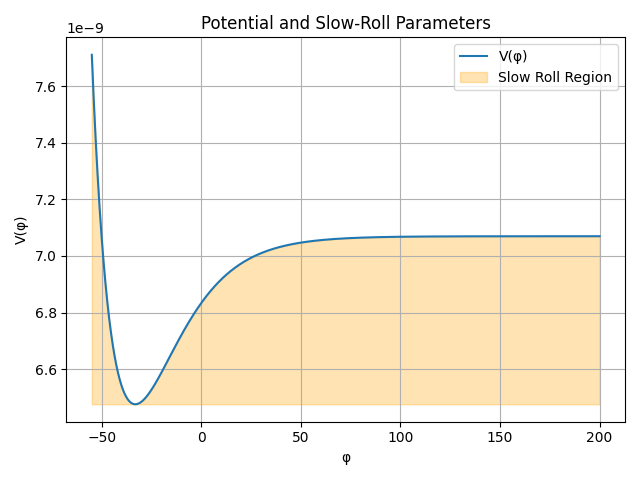
\includegraphics[width=0.7\textwidth]{Python/Figures/New Potenial with gravity.png}
    \caption{The second case graphed, values listed below}
    \label{New potential}
\end{figure}

Here,

$\mu = 1    ,M = 20     ,\phi_0 = 3   .\gamma = 20 ,\alpha = -50,\beta = 1 ,K = 1, C = -2  $
where $K = \sqrt{\frac{k-6}{2}}$. Plotting $\varphi$ vs N also gives us a straight line.

I have also found, there can be old inflation kind of graphs with a suitable choice of parameters, as graphed below,


\begin{comment}
\begin{figure}[h!]
    \centering
    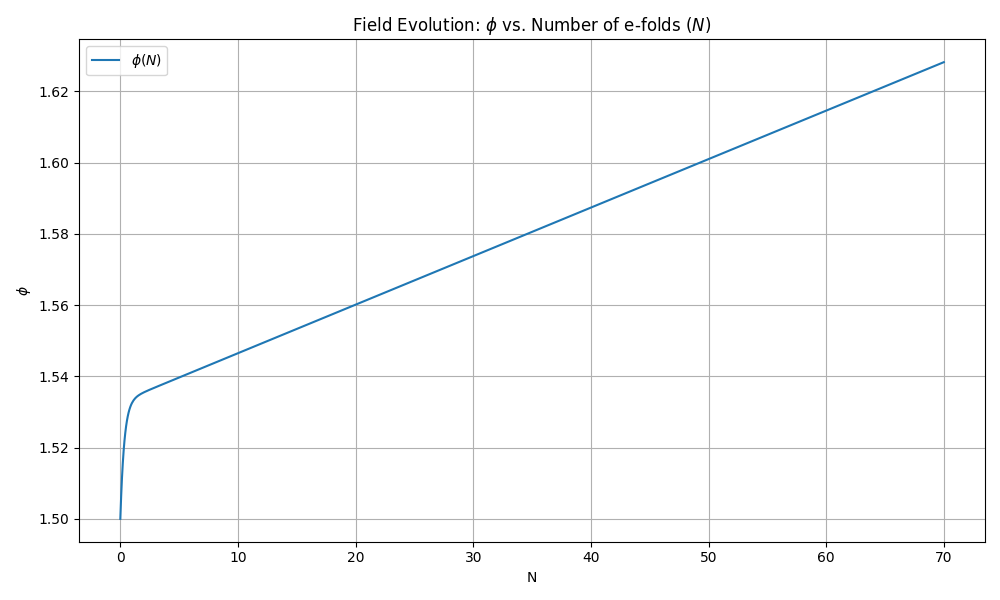
\includegraphics[width=0.6\textwidth]{Python/Figures/NewField as a function of N.png}
    \caption{Newfield as func of N}
    \label{Newfield as func of N}
\end{figure}
\end{comment}

\textbf{FOR CASE I, If $D < 0$ };
\begin{figure}[h!]
    \centering
    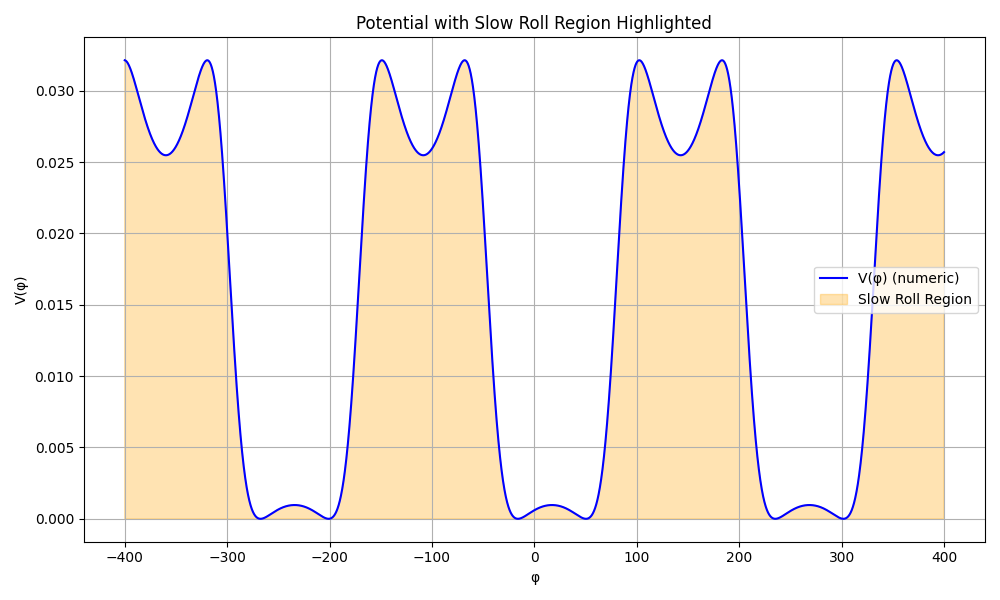
\includegraphics[width=0.7\textwidth]{Python/Figures/New Potenial CASE I with gravity.png}
    \caption{Newfield V1.5 Potential (CASE I)}
    \label{Newfield V1.5 as func of N}
\end{figure}

Maybe total potential (no approx) is like a series of both? So multiple valleys and plateaus and continuously rising. Taylor expand?

\begin{equation}
    \mathcal{L}_{inflaton} = \frac{M^2}{2} \left[-\frac{36\beta}{A} + \frac{\phi_0^2 (\gamma^2 - 4\beta\alpha)(k-6)}{2 A^2}\right] (\partial_\mu \varphi \partial^\mu \varphi) -  \frac{1}{A^2} \frac{\mu^2}{2} \phi^2_0 \varphi^2 
\end{equation}

\section{Equations of Motion for my Action (Nonconstant Derivative coupling)}
Method using \cite{Baumann_2022} (but original derivation)  
So action is

\begin{equation} \label{44}
    S = \int \text{dt}\text{d}^3\text{x} \; \text{a}^3(t) \left[ \frac{K(\varphi)}{2}(\dot{\varphi}^2 - (\grad \varphi)^2) - V(\varphi) \right]
\end{equation}

where,
\begin{align}
    K(\varphi) &= M^2 \left[-\frac{36\beta}{A} + \frac{\phi_0^2 (\gamma^2 - 4\beta\alpha)(k-6)}{2 A^2}\right] \nonumber \\
    V(\varphi) &=  \frac{\mu^2 \phi_0^2 \varphi^2}{2 A^2}
\end{align}
where $A = (\beta \varphi^2  +\gamma \phi_0 \varphi +\alpha \phi^2_0)$

\textbf{NOTE : By mistake, I have taken M to be $M_p/\sqrt{2}$, its fine tho}

varying eqn \ref{44} (and neglecting the grad term cause homogenous fluid), we get

\begin{align}
    \delta S &= \int \text{dt}\,\text{d}^3\text{x} \;  \left[ a^3K_{,\varphi} \frac{\dot{\varphi}^2}{2} \delta \varphi + a^3 K \dot{\varphi} \dot{\delta \varphi} - a^3V_{,\varphi} \delta\varphi \right] \nonumber \\
    &\Rightarrow \int \text{dt}\,\text{d}^3\text{x} \;  \left[ a^3K_{,\varphi} \frac{\dot{\varphi}^2}{2} \delta \varphi - \frac{\text{d}}{\text{d}t}(a^3 K \dot{\varphi}) \delta \varphi - a^3V_{,\varphi} \delta\varphi \right] \nonumber \\
    &\Rightarrow \int \text{dt}\,\text{d}^3\text{x} \;  \left[ a^3K_{,\varphi} \frac{\dot{\varphi}^2}{2}  -  3\dot{a} a^2 K \dot{\varphi} - a^3 K_{,\varphi}\dot{\varphi}^2 - a^3 K \ddot{\varphi} - a^3V_{,\varphi}  \right]\delta \varphi
    \nonumber \\
    &\Rightarrow \int \text{dt}\,\text{d}^3\text{x} \; - \left[ a^3 K \ddot{\varphi} + a^3K_{,\varphi} \frac{\dot{\varphi}^2}{2}  +  3\dot{a} a^2 K \dot{\varphi} + a^3V_{,\varphi}  \right]\delta \varphi
\end{align}

Setting the variation inside to zero, we get

\begin{equation} \label{47}
    K \ddot{\varphi} + \dot{\varphi} \left(\frac{K_{,\varphi} \dot{\varphi}}{2} + 3H K \right) + V_{,\varphi}   = 0
\end{equation}

Simple crosscheck, if $K = 1$, we get $ \ddot{\varphi} +  3H \dot{\varphi}  + V_{,\varphi}   = 0$, which is correct EOM for inflaton field
YAYYY GOT IT

So we can readoff the energy density and pressure to be,

\begin{align}
    \rho &= \frac{K(\varphi)}{2} \dot{\varphi}^2 + V(\varphi) \nonumber \\
    p &= \frac{K(\varphi)}{2} \dot{\varphi}^2 - V(\varphi)
\end{align}

The second friedmann equation $H^2 = \frac{8 \pi G}{3} \rho$, then reads, 

\begin{equation}    \label{Friedmann Eqn 2}
    3 M_p^2H^2 = \frac{K(\varphi)}{2} \dot{\varphi}^2 + V(\varphi)
\end{equation}
differentiate this wrt time

\begin{align}   
     6 M_p^2H \dot{H} &= \frac{K_{,\varphi}}{2} \dot{\varphi}^3 + K \dot{\varphi} \ddot{\varphi} + V_{,\varphi} \dot{\varphi} \nonumber \\
     \Rightarrow 6 M_p^2H \dot{H} &= \frac{K_{,\varphi}}{2} \dot{\varphi}^3 + \dot{\varphi} (K  \ddot{\varphi} + V_{,\varphi}) 
\end{align}

Subbing in from \ref{47}, we get

\begin{align}   \label{51}
    6 M_p^2H \dot{H} &= \frac{K_{,\varphi}}{2} \dot{\varphi}^3 - \dot{\varphi}^2 \left(\frac{K_{,\varphi} \dot{\varphi}}{2} + 3H K \right) \nonumber \\
    \Rightarrow 6 M_p^2H \dot{H} &= - 3H K \dot{\varphi}^2   \nonumber \\ 
    \Rightarrow 2 M_p^2 \dot{H} &= -  K \dot{\varphi}^2
\end{align}

Now, to find the the differential equation of the field $\varphi$ as a function of N, we use $\text{d}N = H \text{d}t$ in eqn \ref{47}, so first $ \dot{\varphi} = H \frac{\text{d}\varphi}{\text{d}N}$, also sub in \ref{51} ($\dot{H} = -  \frac{K}{2 M_p^2 } \left(H \frac{\text{d}\varphi}{\text{d}N} \right)^2$) and then for first term of \ref{47}:

\begin{align} \label{52}
    K \frac{\text{d}^2\varphi}{\text{d}t^2} &= K (H^2 \frac{\text{d}^2\varphi}{\text{d}N^2} + \frac{\text{d}\varphi}{\text{d}N}\dot{H}) \nonumber \\
    \Rightarrow K \ddot{\varphi} &= K H^2 \left( \frac{\text{d}^2\varphi}{\text{d}N^2} - \frac{K}{2M_p^2} \left(\frac{\text{d}\varphi}{\text{d}N} \right)^3 \right) 
\end{align}

For the second term of \ref{47}, we have, 
\begin{align}
    \dot{\varphi} \left(\frac{K_{,\varphi} \dot{\varphi}}{2} + 3H K \right) = H^2 \frac{\text{d}\varphi}{\text{d}N} \left(\frac{K_{,\varphi}}{2} \frac{\text{d}\varphi}{\text{d}N}+ 3 K \right)
\end{align}

and the potential for the third term is, by eqn \ref{Friedmann Eqn 2}

\begin{equation}
    V(\varphi) = H^2 \left( 3 M_p^2 - \frac{K}{2} \left(\frac{\text{d}\varphi}{\text{d}N} \right)^2 \right)
\end{equation}

Putting it all together in the EOM \ref{47}, we get, 

\begin{align}
    K \left( \frac{\text{d}^2\varphi}{\text{d}N^2} - \frac{K}{2M_p^2} \left(\frac{\text{d}\varphi}{\text{d}N} \right)^3 \right) +  \frac{\text{d}\varphi}{\text{d}N} \left(\frac{K_{,\varphi}}{2} \frac{\text{d}\varphi}{\text{d}N}+ 3 K \right) + \left( 3 M_p^2 - \frac{K}{2} \left(\frac{\text{d}\varphi}{\text{d}N} \right)^2 \right) \frac{\text{d}\ln \text{V}(\varphi)}{\text{d} \varphi} &= 0 \nonumber \\
    \Rightarrow K\frac{\text{d}^2\varphi}{\text{d}N^2} +3 K \frac{\text{d}\varphi}{\text{d}N}  - \frac{K^2}{2M_p^2} \left(\frac{\text{d}\varphi}{\text{d}N} \right)^3  +  \frac{K_{,\varphi}}{2}  \left(\frac{\text{d}\varphi}{\text{d}N} \right)^2 +  \left( 3 M_p^2 - \frac{K}{2} \left(\frac{\text{d}\varphi}{\text{d}N} \right)^2 \right) \frac{\text{d}\ln \text{V}(\varphi)}{\text{d} \varphi} &= 0    
\end{align}
\textbf{NO NEED FOR A $R^2$ TERM!!! TAKEN CARE OF HERE!}


which aligns exactly with the equation in \cite{barker2024inflationarygravitationalwavesignatures}, when $K = 1$

so for the values listed below I got the below graph of $\varphi(\text{N}) \: \text{vs} \: \text{N}$,

$\mu = 1, M = 20  ,M_p = \sqrt2 M ,\phi_0 = 3, \gamma = 20 ,\alpha = -50 ,\beta = 1 ,k = 1000$

\begin{figure}[h!]
    \centering
    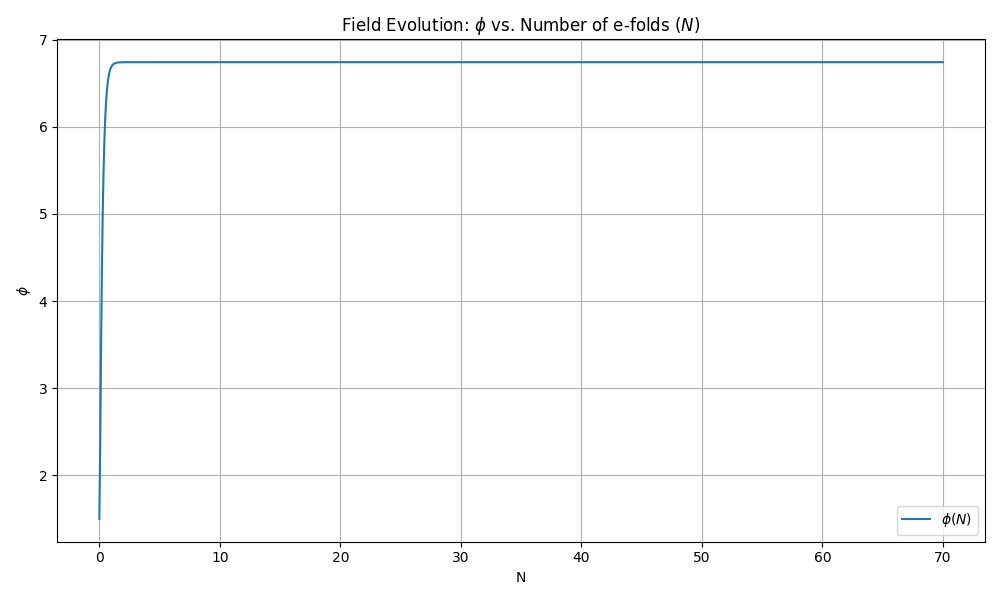
\includegraphics[width=0.7\textwidth]{Python/Figures/New Field as a function of N.png}
    \caption{Newfield as func of N}
    \label{Newfield as func of N}
\end{figure}

and for these values, since $k \gg 1 \implies$ only second term of kinetic coefficient important, I get a similar looking potential (for full lagrangian) 


\begin{figure}[h!]
    \centering
    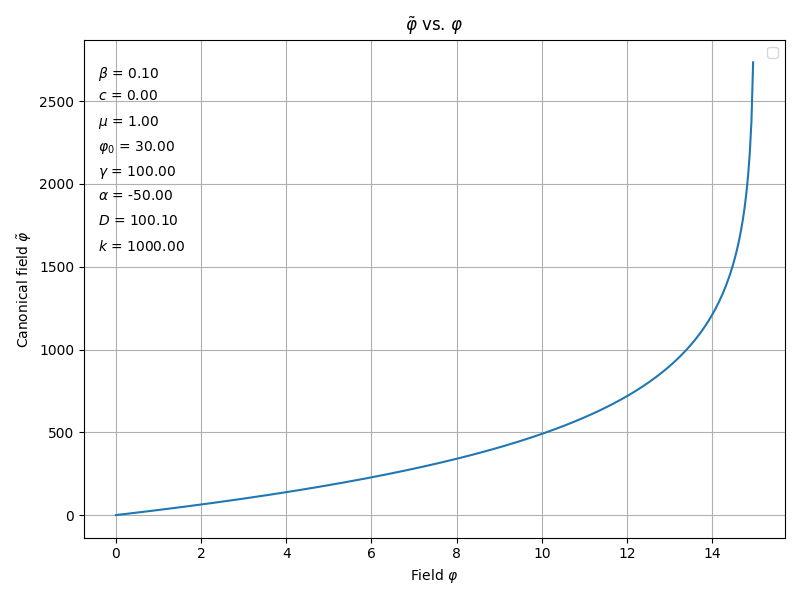
\includegraphics[width=0.7\textwidth]{Python/Figures/Field vs Canonical Field.png}
    \caption{$\tilde{\varphi}$ vs $\varphi$}
    \label{Canonical field vs field}
\end{figure}

\begin{figure}[h!]
    \centering
    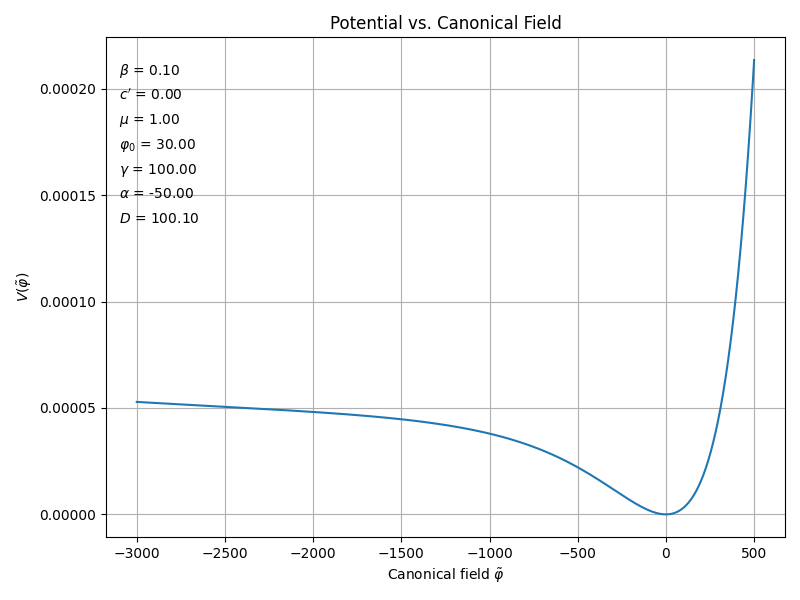
\includegraphics[width=0.7\textwidth]{Python/Figures/Full Lagrangian potential.png}
    \caption{Full lagrangian potential, (blue is potential, rest are derivatives, will add label later)}
    \label{Full lagrangian potential}
\end{figure}




for plateau : $\mu = 1, M = 20  ,M_p = \sqrt2 M ,\phi_0 = 30, \gamma = 100 ,\alpha = -50 ,\beta = 0.1 ,k = 1000$

so by investigations, increasing $\gamma$ now increases length of plateau. Sincce $k \gg 1 \implies$ almost case II inflation, we get that kinda graph.



also, slow roll parameters as a function of N are: 

\begin{figure}[h!]
    \centering
    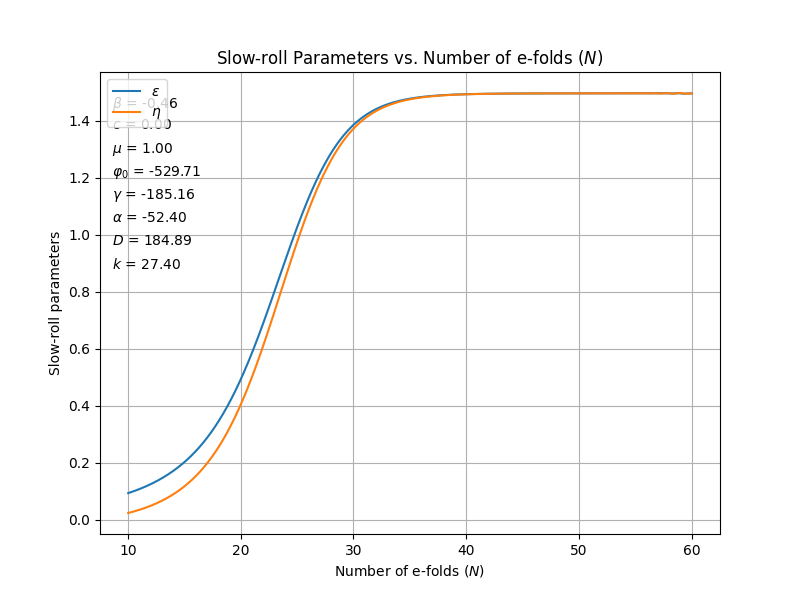
\includegraphics[width=0.7\textwidth]{Python/Figures/Full Slow Roll Parameters as Func of N.png}
    \caption{Hubble Slow Roll Parameters as a function of N}
    \label{Hubble Slow Roll Parameters as a function of N}
\end{figure}

\section{Reduction to the Starobinsky Model}

\begin{align} \label{28a}
    S =\int \text{d}^4\text{x} \; \sqrt{-g} &\; \left[ ( \beta \varphi^2 + \gamma \phi \varphi +\alpha \phi^2) R - 6( \beta \varphi^2 + \gamma \phi \varphi +\alpha \phi^2) (B_{\mu} B^{\mu} - \nabla_\mu B^\mu) \right. \nonumber \\
    &\quad \left. +\frac{\epsilon}{2} D_{\mu}\varphi D^{\mu}\varphi + \frac{\sigma}{2} D_{\mu}\varphi D^{\mu}\phi + \frac{\nu}{2} D_{\mu}\phi D^{\mu}\phi \right. \left. - \frac{\mu^2}{2} \phi^2 \varphi^2 + \frac{\lambda}{2} \varphi^4 + \frac{\kappa}{2} \phi^4 - \frac{\xi}{16} H_{\mu\nu}H^{\mu\nu} \right]  
\end{align}

Let us ignore all other terms except for $R$ coefficient $\varphi^2$ and the $\varphi^4$ terms. 

\begin{equation}
    \begin{aligned}
        \mathcal{L} &= (\alpha \phi^2_0 + \beta \varphi^2 + \gamma \phi_0 \varphi) (R - 6B_{\mu} B^{\mu} - 6\nabla_\mu B^\mu) \\
        &+ \frac{\epsilon}{2} (\partial_\mu \varphi - (\varphi + \frac{\sigma}{\epsilon} \phi_0)B_\mu)(\partial^\mu \varphi - \varphi B^\mu)\\
        &- \frac{\mu^2}{2} \phi^2_0 \varphi^2 + \frac{\nu \phi_{0}^{2}}{2} B_\mu B^\mu - \frac{\xi}{16} H_{\mu\nu}H^{\mu\nu}
    \end{aligned}
\end{equation}

\begin{equation}
    \mathcal{L} = \beta \varphi^2 R - 6\beta \varphi^2 B_\mu B^\mu + 6\partial_\mu(\beta \varphi^2) B^\mu - \frac{\epsilon}{2} (\partial_\mu \varphi - (\varphi + \frac{\sigma}{\epsilon} \phi_0)B_\mu)(\partial^\mu \varphi - \varphi B^\mu) + \frac{\nu \phi_0^2}{2} B^\mu B_\mu
\end{equation}

eom for 


\begin{equation}
    \tilde{R} = \Omega^{-2} \left[ R - 6 \Box(\ln \Omega) - \frac{6 g^{\alpha \beta} \nabla_\alpha\Omega \nabla_\beta\Omega}{\Omega^2} \right]
\end{equation}


\section{Random Lagrangian Try (Not relevant)}
\begin{equation}
    \mathcal{L} = K(\phi) \left[\frac{1}{2} \partial_\mu\phi\partial^\mu\phi - V(\phi) \right]
\end{equation}
The Euler Lagrange eqns read:
\begin{equation}
    \partial^\mu (K \partial_\mu\phi) + K_{,\phi} (\frac{1}{2} \partial_\mu\phi\partial^\mu\phi - V(\phi)) + K V_{,\phi} = 0
\end{equation}
So
\begin{equation}
    K \partial^\mu \partial_\mu\phi + K_{,\phi} (\frac{3}{2} \partial_\mu\phi\partial^\mu\phi - V(\phi)) + K V_{,\phi} = 0
\end{equation}


\begin{equation}
     \partial^\mu \partial_\mu\phi + V_{,\phi}  = (T_\mu^\mu) \frac{\text{d}}{\text{d}\phi} \ln (K(\phi)) 
\end{equation}



\newpage

\section{Slicing Spacetime}

At each point $p$ in spacetime

Given that the FLRW metric considers a homogeneous and isotropic spacetime, a natural choice to analyse the metric and dynamics of this space would be to slice the 4D spacetime ($\mathcal{M}_4$) into a time-ordered sequence of 3D spacelike hypersurfaces $\Sigma_t$ such that on the hypersurface, time is constant \cite{baumann2012tasilecturesinflation},\cite{gourgoulhon_31_2007}:
\begin{equation}
    \forall t \in \mathbb{R} : \Sigma_t = \{p \in \mathcal{M}_4 ; \hat{t} (p) = t\}
\end{equation}
Since $t$ is always increasing and we want this slicing to cover all of spacetime, we also have:


\section{Reduction to the Starobinsky Model} \label{Appendix B}

The Starobinsky Model \cite{STAROBINSKY198099} Lagrangian includes a quadratic curvature (a scale-invariant) term in the Einstein-Hilbert action. When the curvature is high, the quadratic term dominates and drives inflation away from an unstable de Sitter fixed point \cite{Cecchini_2024}. Looking at a particular sector in our theory from Lagrangian \ref{32a} where we have chosen $\lambda = \beta$,
\begin{equation} \label{B1}
    S =\int \text{d}^4\text{x} \sqrt{-g} \left[ (\alpha \phi_0^2 + \beta \varphi^2)\mathcal{R} - \frac{\lambda}{2} \varphi^4 \right]  
\end{equation}
Upon utilization of the Euler-Lagrange equation on the $\varphi$ field $2 \beta \varphi R - 2\beta \varphi^3 = 0$, if $\varphi \neq 0$, the other solution $\varphi^2 = R$, gives us \ref{B2}. This can be re-written as:
\begin{equation} \label{B2}
    S =\int \text{d}^4\text{x} \sqrt{-g} \left[ \alpha \phi_0^2 \mathcal{R} + \frac{\beta}{2} \mathcal{R}^2  \right]
\end{equation}
 We can see that this action, a particular regime of the general lagrangian \ref{32a}, is equivalent to the Starobinsky model. Therefore, to match this with our model, we use our variable dictionary \ref{35}

To reduce to the above equations to \ref{B2}, we choose: $\gamma = 0, k = -12$, and $\beta$ negative, giving $\epsilon = \sigma = \nu = 0$. Our $K(\varphi)$ and $V(\varphi)$ given in \ref{37} and \ref{38} therefore reduce to:
\begin{align}
    \text{K}(\varphi) &= \left[\frac{12 M^2 \beta^2 \varphi^2}{ (\beta \varphi^2 + \alpha \phi_0^2)^2}\right] \\
    \text{V}(\varphi) &= \frac{ M^4 \lambda \varphi^4}{2(\beta \varphi^2 + \alpha \phi_0^2)^2}    
\end{align}
Giving the field redefinition:
\begin{align}
    \tilde{\varphi}(\varphi) &= \sqrt{3}M \ln\left(1 + \frac{\beta \varphi^2}{\alpha \phi_0^2} \right) \nonumber \\
    \varphi^2(\tilde{\varphi}) &=  \frac{\alpha}{\beta} \phi_0^2\left [ \exp\left(\frac{\tilde{\varphi}}{\sqrt{3}M}\right) -1\right]
\end{align}
Using this in the potential, we get reproduce the famous Starobinsky formula:
\begin{equation}
    \text{V}(\tilde{\varphi}) = \frac{ M_p^4}{8 \beta}  \left(1 - \exp\left(-\sqrt{\frac{2}{3}}\frac{ \tilde{\varphi}}{ M_p}\right)\right)^2
\end{equation}
This is the exact Starobinsky potential \cite{STAROBINSKY198099}, \cite{maeda_inflation_1988}. In comparison with the Starobinsky Model, \cite{ivanov2022analytic}, \cite{lust2024starobinsky}, we see that the parameters $m^2 \approx \frac{3}{4} 10^{-10}M_p^2 =\frac{M_p^2}{8\beta}$, giving us $\beta \approx 10^{9}$. We also note that the terms $\alpha, \phi_0$ drop out of the final potential, giving us the Starobinsky behaviour of a one-parameter potential.

\section{Reduction to Barker Model}
For the Lagrangian \ref{32a} to reduce to Barker, we require $\beta = \gamma =0$; this can be done through the choice $k \rightarrow\infty$. To ensure that the conformal transformation we did on the way is not singular, we require $\alpha$ finite. Converting the parameters from $\alpha, \beta, \gamma$ to $\epsilon, \sigma, \nu$ in the $K,V$ formulae: \cite{caputa_cosmology_2013}

We get:
\begin{align}
    \text{K}(\varphi) &= \left[\frac{M^2 \phi_0^2 (\sigma^2 - 4\epsilon\nu)k}{2 (\epsilon \varphi^2 + \sigma\phi_0\varphi + \nu \phi_0^2)^2}\right] \label{C4}  \\
    \text{V}(\varphi) &= \frac{ k^2 M^4 \mu^2 \phi^2_0 \varphi^2}{2(\epsilon \varphi^2 + \sigma\phi_0\varphi + \nu \phi_0^2)^2}
\end{align}
In the limit $k \rightarrow\infty$, the field redefinition becomes:
\begin{equation}
    \varphi(\tilde{\varphi}) = \frac{\phi_0}{2\epsilon} \left[\sigma - \sqrt{\sigma^2 - 4\epsilon \nu} \tanh\left(\frac{\tilde{\varphi}}{M_p\sqrt{k}}-c \right) \right]
\end{equation}
The field $\varphi$ is bounded by:
\begin{equation}
    \frac{\phi_0}{2\epsilon} \left[\sigma - \sqrt{\sigma^2 - 4\epsilon \nu}\right] < \varphi < \frac{\phi_0}{2\epsilon} \left[\sigma + \sqrt{\sigma^2 - 4\epsilon \nu}  \right]
\end{equation}


\subsubsection{\textbf{CASE I }: $k \gg 1$}

Assuming $\beta \ll \phi_0^2(4\alpha\beta - \gamma^2)(k+6)$, we get the field redefinition ($\gamma^2 <4\alpha\beta$) and using $D = \sqrt{4\alpha\beta-\gamma^2}$:
\begin{equation}
    \frac{d\tilde{\varphi}}{d\varphi} = \left[ \sqrt{\frac{k}{2}} \frac{M \phi_0 D}{\beta \varphi^2  +\gamma \phi_0 \varphi +\alpha \phi^2_0} \right]
\end{equation}
This gives:
\begin{equation}
    \varphi(\tilde{\varphi}) = \frac{\phi_0}{2\beta} \left[ \sqrt{4\alpha \beta - \gamma^2} \tan\left(\frac{\tilde{\varphi}}{M_p\sqrt{k}}-c \right) -\gamma \right]
\end{equation}
Using this in the potential (keeping only the $\mu$ term), we get:
\begin{equation}
    V(\tilde{\varphi}) =  \frac{\mu^2 M_p^4}{2(4\alpha\beta-\gamma^2)^2} \cos^4(X)  \left [ \gamma - \sqrt{4\alpha\beta- \gamma^2} \tan(X)\right]^2
\end{equation}
Where $X = \left(\left(\frac{\tilde{\varphi}}{\sqrt{k}M_p}\right) - c\right)$
Plotting this potential and keeping $c = 0$, we get figure \ref{CASE I potential (HillTop Potential)}, which is a hilltop potential \cite{boubekeur_hilltop_2005}. 
\begin{figure}[h!]
    \centering
    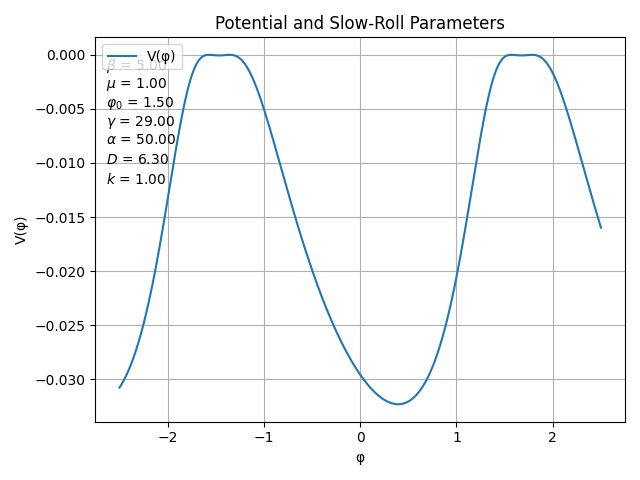
\includegraphics[width=0.4\textwidth]{Python/Figures/Case1 Potential.png}
    \caption{CASE I}
    \label{CASE I potential (HillTop Potential)}
\end{figure}

\subsubsection{\textbf{CASE II}: $k = -6$}
Assuming $k=-6$,  we get the field redefinition:
\begin{equation}
    \frac{d\tilde{\varphi}}{d\varphi} = \sqrt{\left[\frac{12\beta M^2}{(\beta \varphi^2 + \gamma\phi_0\varphi + \alpha \phi_0^2)} \right]}
\end{equation}
For the field redefinition to make sense, we require $\gamma^2 < 4\alpha \beta$, this gives us:
\begin{equation}
    \varphi(\tilde{\varphi}) = \frac{1}{4\beta} \left(\text{e}^{-X}(\text{e}^{2X} - 2\text{e}^X \gamma \phi_0 - \phi_0^2(4\alpha\beta-\gamma^2)) \right)
\end{equation}
Where, $X = \frac{\tilde{\varphi}}{\sqrt{6}M_p}+c$The resulting potential is:
\begin{equation}
    V(\tilde{\varphi}) =  \frac{2 \mu ^2 M_p^4 e^{2 X} \phi_0^2 \left(\text{e}^{2X} - 2\text{e}^X \gamma \phi_0 - \phi_0^2(4\alpha\beta-\gamma^2)\right)^2}{\left(\phi ^2 \left(4 \alpha  \beta -\gamma ^2\right)+\text{e}^{2 X}\right)^4}
\end{equation}
Where $X(\tilde{\varphi}) = \frac{\tilde{\varphi}}{3\sqrt{2}M_p}$. The graph for the same is below.

\begin{figure}[h!]
    \centering
    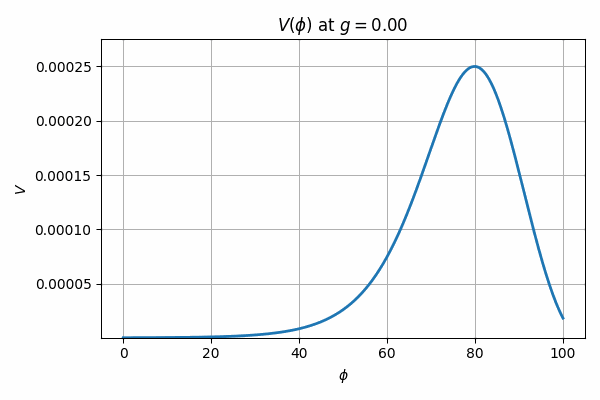
\includegraphics[width=0.4\textwidth]{Python/Figures/potential_vs_g.png}
    \caption{CASE II}
    \label{CASE II potential (Exponential)}
\end{figure}


\subsection{\textbf{NUMERICAL ANALYSIS}}
Stitching together the two regimes, we can see that $K(\varphi)$ interpolates between the two regimes based on values of $\varphi \, \, \text{and}\, \,k$. For intermediate $k$, both terms contribute, leading to a non-trivial kinetic structure, which is not always integrable.

For $\varphi \rightarrow 0$, the $\frac{1}{A^2(\varphi)}$ term dominates, giving a tangent contribution, a power-law structure/steep potential close to zero. For $\varphi \rightarrow \infty$, the $\frac{1}{A(\varphi)}$ term dominates,  giving a hyperbolic sine contribution, providing an exponentially damped solution leading to a plateau-like shape. 

Finally, using Python, we can numerically integrate equation \ref{40}, interpolate the function $\tilde{\varphi}(\varphi)$, invert it, and use it to attain the shape of the true potential \ref{38}. The parameters below have been chosen such that the scalar spectral index $n_s = 1 + 2\eta_V - 6 \epsilon_V$ (We would have used $n_s = 1 + \frac{1}{K}(2\eta_V - 6 \epsilon_V -\sqrt{2\epsilon_V}\lambda_K)$ ($\lambda_K = M_p \frac{K_{,\varphi}}{K}$), if the definitions of our slow roll parameters were canonical, but since we have accounted for it's non canonical nature in \ref{26} and \ref{29}, we can use the normal definition \cite{chung2003running} ),  is close to the experimental value of 0.968 at around 60 efolds.


\printbibliography

\end{document}

